\documentclass{article}
\usepackage[utf8]{inputenc}
\usepackage{amsmath}
\usepackage{listings}
\usepackage{graphicx}

\title{CIS 419/519: Homework 2}
\author{\{Your name here\}}
\date{}

\begin{document}

\maketitle
    Although the solutions are my own, I consulted with the following people while working on this homework: \{Names here\} \\

\begin{enumerate}
    \item[\textbf{4.1.1}]
    Winnow hyperparameter sweep:
    \begin{center}
        \begin{tabular}{|c|c|c|}
            \hline
            $\alpha$ & Sparse & Dense \\
            \hline
            1.1 & & \\
            1.01 & & \\
            1.005 & & \\
            1.0005 & & \\
            1.0001 & & \\
            \hline
        \end{tabular}
    \end{center}

    Averaged Winnow hyperparameter sweep:
    \begin{center}
        \begin{tabular}{|c|c|c|}
            \hline
            $\alpha$ & Sparse & Dense \\
            \hline
            1.1 & & \\
            1.01 & & \\
            1.005 & & \\
            1.0005 & & \\
            1.0001 & & \\
            \hline
        \end{tabular}
    \end{center}

    Perceptron with AdaGrad hyperparameter sweep:
    \begin{center}
        \begin{tabular}{|c|c|c|}
            \hline
            $\eta$ & Sparse & Dense \\
            \hline
            1.5 & & \\
            0.25 & & \\
            0.03 & & \\
            0.005 & & \\
            0.001 & & \\
            \hline
        \end{tabular}
    \end{center}

    Averaged Perceptron with AdaGrad hyperparameter sweep:
    \begin{center}
        \begin{tabular}{|c|c|c|}
            \hline
            $\eta$ & Sparse & Dense \\
            \hline
            1.5 & & \\
            0.25 & & \\
            0.03 & & \\
            0.005 & & \\
            0.001 & & \\
            \hline
        \end{tabular}
    \end{center}

    \item[\textbf{4.1.2}]
    Sparse learning curves:
    \begin{center}
        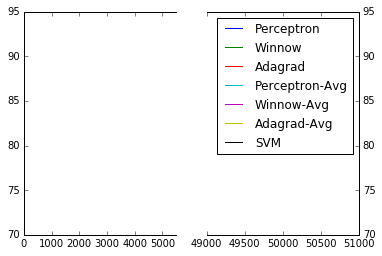
\includegraphics[]{sample.png}
    \end{center}

    Dense learning curves:
    \begin{center}
        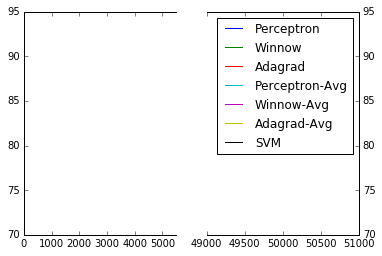
\includegraphics[]{sample.png}
    \end{center}

    \begin{enumerate}
        \item Answer to question 1
        \item Answer to question 2
    \end{enumerate}

    \item[\textbf{4.1.3}]
    Final test accuracies
    \begin{center}
        \begin{tabular}{|c|c|c|}
            \hline
            Model & Sparse & Dense \\
            \hline
            Perceptron & & \\
            Winnow & & \\
            Perceptron with AdaGrad & & \\
            Averaged Perceptron & & \\
            Averaged Winnow & & \\
            Averaged Perceptron with AdaGrad & & \\
            SVM & & \\
            \hline
        \end{tabular}
    \end{center}

    \item[\textbf{4.1.4}]
    Extra credit. Insert your plot(s) if you do this problem

    \item[\textbf{4.2}]
    CoNLL and Enron F$_1$ scores:
    \begin{center}
        \begin{tabular}{|c|c|c|}
            \hline
            Model & CoNLL Test F$_1$ & Enron Test F$_1$ \\
            \hline
            Averaged Perceptron & & \\
            SVM & & \\
            \hline
        \end{tabular}
    \end{center}
    Discussion of the F$_1$ scores and whether or not they're different with an explanation why.

\end{enumerate}
\end{document}
